%%%%%%%%%%%%%%%%%%%%%%%%%%%%%%%%%%%%%%%%%%%%%%%%%%%%%%%%%%%%%%%%%%%%%%%%%%% 
% 
% Generic template for the anteproyectos of TFC/TFM/TFGs
% 
% $Id: anteproyecto.tex,v 1.6 2018/09/11 12:23:48 macias Exp $
% 
% By:
%  + Javier Macías-Guarasa. 
%    Departamento de Electrónica
%    Universidad de Alcalá
%  + Roberto Barra-Chicote. 
%    Departamento de Ingeniería Electrónica
%    Universidad Politécnica de Madrid   
% 
% Based on original sources by Roberto Barra, Manuel Ocaña, Jesús Nuevo,
% Pedro Revenga, Fernando Herránz and Noelia Hernández. Thanks a lot to
% all of them, and to the many anonymous contributors found (thanks to
% google) that provided help in setting all this up.
% 
% See also the additionalContributors.txt file to check the name of
% additional contributors to this work.
% 
% If you think you can add pieces of relevant/useful examples,
% improvements, please contact us at (macias@depeca.uah.es)
% 
% You can freely use this template and please contribute with
% comments or suggestions!!!
% 
%%%%%%%%%%%%%%%%%%%%%%%%%%%%%%%%%%%%%%%%%%%%%%%%%%%%%%%%%%%%%%%%%%%%%%%%%%% 

% This is for rubber to clean additional files
% rubber: clean anteproyecto.acn anteproyecto.acr anteproyecto.alg anteproyecto.cod anteproyecto.ist anteproyecto.out anteproyecto.sbl anteproyecto.slg anteproyecto.sym anteproyecto.lor

\documentclass[11pt,a4paper,oneside]{article}

%%%%%%%%%%%%%%%%%%%%%%%%%%%%%%%%%%%%%%%%%%%%%%%%%%%%%%%%%%%%%%%%%%%%%%%%%%% 
% BEGIN Preamble and configuration section
% 
\input{../Config/preamble.tex}    % DO NOT TOUCH THIS LINE. You can edit
                                  % the file to modify some default settings

\input{../Config/myconfig.tex}    % DO NOT TOUCH THIS LINE, but EDIT THIS FILE
                                  % to set your specific settings (related
                                  % to the document language, your degree,
                                  % document details (such as title, author
                                  % (you), your email, name of the tribunal
                                  % members, document year, keyword and
                                  % palabras clave) and link colors), and
                                  % define your commonly used commands
                                  % (some examples are provided).

\input{../Config/postamble.tex}   % DO NOT TOUCH THIS LINE. Yes, I know,
                                  % "postamble" is not a valid word... :-)
%
% END Preamble and configuration section
%%%%%%%%%%%%%%%%%%%%%%%%%%%%%%%%%%%%%%%%%%%%%%%%%%%%%%%%%%%%%%%%%%%%%%%%%%%

% path to directories containing images
\graphicspath{{../Book/logos/}{../Book/figures/}{../Book/diagrams/}} % Edit this to your
                                  % needs. Only logos is really required
                                  % when you generate your own content.
% 
% END Preamble and configuration section
%%%%%%%%%%%%%%%%%%%%%%%%%%%%%%%%%%%%%%%%%%%%%%%%%%%%%%%%%%%%%%%%%%%%%%%%%%% 

\title{Anteproyecto de \myWorkTypeFull}        % DO NOT TOUCH THIS LINE
\date{\myThesisProposalDate}                         % DO NOT TOUCH THIS LINE
\author{\myAuthorFullName}

%%%%%%%%%%%%%%%%%%%%%%%%%%%%%%%%%%%%%%%%%%%%%%%%%%%%%%%%%%%%%%%%%%%%%%%%%%% 
% Let's start with the real stuff
%%%%%%%%%%%%%%%%%%%%%%%%%%%%%%%%%%%%%%%%%%%%%%%%%%%%%%%%%%%%%%%%%%%%%%%%%%% 
\begin{document}                                   % DO NOT TOUCH THIS LINE

%%%%%%%%%%%%%%%%%%%%%%%%%%%%%%%%%%%%%%%%%%%%%%%%%%%%%%%%%%%%%%%%%%%%%%%%%%% 
% BEGIN within-document configuration, frontpage and cover pages generation
% 

% Set Language dependent issues that must be set after \begin{document}
\input{../Config/setlanguagedependentissues.tex} % DO NOT TOUCH THIS LINE
                                                 % NOR THE FILE

% 
% END within-document configuration, frontpage and cover pages generation
%%%%%%%%%%%%%%%%%%%%%%%%%%%%%%%%%%%%%%%%%%%%%%%%%%%%%%%%%%%%%%%%%%%%%%%%%%% 

\maketitle

\begin{description}                               % DO NOT TOUCH THIS LINE
\item[\expandafter\makefirstuc\expandafter{\wordAutorOrAutora}:] \myAuthorFullName                       % DO NOT TOUCH THIS LINE
\item[\expandafter\makefirstuc\expandafter{\wordTutorOrTutores}:] \myAdvisors                   % DO NOT TOUCH THIS LINE
  \item[Titulación:] \myDegreefull                % DO NOT TOUCH THIS LINE
  \item[Título:] \myBookTitleSpanish              % DO NOT TOUCH THIS LINE
  \ifthenelse{\equal{\myLanguage}{english}}       % DO NOT TOUCH THIS LINE
  {                                               % DO NOT TOUCH THIS LINE
  \item[Título en inglés:] \myBookTitleEnglish    % DO NOT TOUCH THIS LINE
  }                                               % DO NOT TOUCH THIS LINE
  {                                               % DO NOT TOUCH THIS LINE
  }                                               % DO NOT TOUCH THIS LINE
\item[Departamento:] \myDepartment                % DO NOT TOUCH THIS LINE
\end{description}                                 % DO NOT TOUCH THIS LINE

%\tableofcontents

%%%%%%%%%%%%%%%%%%%%%%%%%%%%%%%%%%%%%%%%%%%%%%%%%%%%%%%%%%%%%%%%%%%%%%%%%%% 
%%%%%%%%%%%%%%%%%%%%%%%%%%%%%%%%%%%%%%%%%%%%%%%%%%%%%%%%%%%%%%%%%%%%%%%%%%% 
%%%%%%%%%%%%%%%%%%%%%%%%%%%%%%%%%%%%%%%%%%%%%%%%%%%%%%%%%%%%%%%%%%%%%%%%%%% 
%%%%%%%%%%%%%%%%%%%%%%%%%%%%%%%%%%%%%%%%%%%%%%%%%%%%%%%%%%%%%%%%%%%%%%%%%%% 
%%%%%%%%%%%%%%%%%%%%%%%%%%%%%%%%%%%%%%%%%%%%%%%%%%%%%%%%%%%%%%%%%%%%%%%%%%% 
%%%%%%%%%%%%%%%%%%%%%%%%%%%%%%%%%%%%%%%%%%%%%%%%%%%%%%%%%%%%%%%%%%%%%%%%%%% 
%%%%%%%%%%%%%%%%%%%%%%%%%%%%%%%%%%%%%%%%%%%%%%%%%%%%%%%%%%%%%%%%%%%%%%%%%%% 
% BEGIN Normal sections. Edit/modify all within this section

% Viñetas de las listas: cuadrado negro en el primer nivel, punto en el segundo.
\setlist[itemize,1]{label={\small$\blacksquare$}}
\setlist[itemize,2]{label={\textbullet}}

\section{Introducción}
\label{sec:introduccion}

El consumo energético del software es una problemática de creciente
relevancia en el contexto de la sostenibilidad digital. Aunque se han
producido avances significativos en la eficiencia energética del
hardware, el software raramente se diseña o evalúa teniendo en cuenta su
huella energética. Esta situación tiene un impacto real en el consumo de
los dispositivos de usuario y en la infraestructura de cómputo
global~\cite{verdecchia2021}.

En este contexto, JoularJX es un agente Java de código abierto,
desarrollado en la Universidad de Pau (Francia) por el Dr.~Adel
Noureddine, que permite medir el consumo energético de aplicaciones Java
a nivel de método de forma no intrusiva, sin modificar el código fuente
de la aplicación monitorizada~\cite{joularjx2022}. JoularJX se engancha a
la JVM en el arranque y, mediante muestreo estadístico del
\textit{stacktrace} activo, atribuye a cada método la energía consumida
por el proceso durante su ejecución. Es compatible con Windows, Linux y
macOS, y está activamente mantenida (última versión: 3.1.0, febrero de
2026)~\cite{joularjx3}.

Este Trabajo Fin de Grado propone estudiar JoularJX en profundidad y
aplicarla a un caso de experimentación concreto: la comparación del
consumo energético de Jackson~\cite{jackson} y Gson~\cite{gson}, las dos
librerías Java de procesamiento de JSON más utilizadas. Ambas resuelven
el mismo problema funcional ---serializar y deserializar objetos Java a
formato JSON--- pero con arquitecturas internas radicalmente distintas,
lo que las convierte en un caso de estudio ideal para analizar cómo las
decisiones de diseño del software impactan en su eficiencia
energética~\cite{noureddine2025}.


\section{Objetivos}
\label{sec:objetivos-y-campo}

\subsection*{Objetivo general}

Analizar y evaluar JoularJX como herramienta para la medición del
consumo energético de aplicaciones Java, aplicándola a la comparación de
dos librerías de código abierto ampliamente utilizadas que resuelven el
mismo problema funcional.

\subsection*{Objetivos específicos}

Los objetivos específicos de este proyecto son los siguientes:

\begin{itemize}
\item Comprender cómo mide JoularJX el consumo energético a nivel de
  método Java: arquitectura de agente, muestreo de \textit{stacktrace},
  fuentes de datos (RAPL, Power Monitor para Windows) y formatos de
  salida.

\item Instalar y configurar JoularJX en un entorno Windows~11,
  documentando el proceso paso a paso.

\item Preparar un banco de pruebas reproducible sobre las librerías
  Jackson y Gson que permita medir su consumo energético en operaciones
  equivalentes de serialización y deserialización de JSON.

\item Ejecutar las mediciones con JoularJX, analizar los resultados
  (consumo total, consumo por método y \textit{hotspots} energéticos) y
  comparar ambas librerías.

\item Evaluar las limitaciones de JoularJX: precisión del muestreo,
  \textit{overhead} del agente y variabilidad de las mediciones entre
  ejecuciones.
\end{itemize}

\subsection*{Campo de aplicación}

El TFG se enmarca en el área de ingeniería del software sostenible. Los
resultados son de interés para desarrolladores Java, arquitectos de
software y cualquier organización que quiera tomar decisiones informadas
sobre qué librerías usar en función de su eficiencia energética. El
trabajo no está sujeto a ningún acuerdo de confidencialidad.


\section{Descripción del trabajo}
\label{sec:descr-del-trab}

El trabajo se estructura en tres bloques: estudio teórico de JoularJX,
configuración del entorno experimental y experimentación comparativa
entre Jackson y Gson. Los componentes principales son los siguientes:

\begin{enumerate}

\item \textbf{Estudio de JoularJX.} Revisión de los artículos originales de
  JoularJX~\cite{joularjx2022,joularjx3}, estudio de su arquitectura
  interna como agente Java (API \texttt{java.lang.instrument}),
  mecanismo de muestreo de \textit{stacktrace}, fuentes de energía según
  la plataforma y formato de salida CSV.

\item \textbf{Instalación y configuración del entorno.} Instalación de JoularJX
  (\textit{jar} del agente), de Power Monitor for
  Windows~\cite{winpowermonitor} (lectura de los MSR de RAPL en Windows)
  y configuración del fichero \texttt{config.properties}. Verificación
  del funcionamiento con un programa Java de prueba. Descarga de
  Jackson~\cite{jackson} y Gson~\cite{gson} desde Maven Central.

\item \textbf{Diseño del banco de pruebas.} Diseño de un conjunto de casos de
  prueba equivalentes para ambas librerías: serialización y
  deserialización de objetos simples y complejos, con diferentes tamaños
  de \textit{payload} (pequeño, mediano y grande). Uso de JMH
  (\textit{Java Microbenchmark Harness}) para garantizar condiciones de
  medición estables y reproducibles.

\item \textbf{Experimentación y análisis.} Ejecución de JoularJX sobre ambas
  librerías. Recogida de datos de consumo total (julios), consumo por
  método y evolución temporal. Repetición de las mediciones para
  verificar su estabilidad. Análisis de resultados e identificación de
  \textit{hotspots} energéticos. Comparación normalizada por operación
  (julios por serialización y deserialización).

\end{enumerate}

% NOTA: cuando tengas el diagrama de bloques del sistema, guárdalo en
% Book/diagrams/ o Book/figures/ y descomenta este bloque, cambiando el
% nombre del fichero.
%
% \begin{figure}[tphb]
%   \centering
%   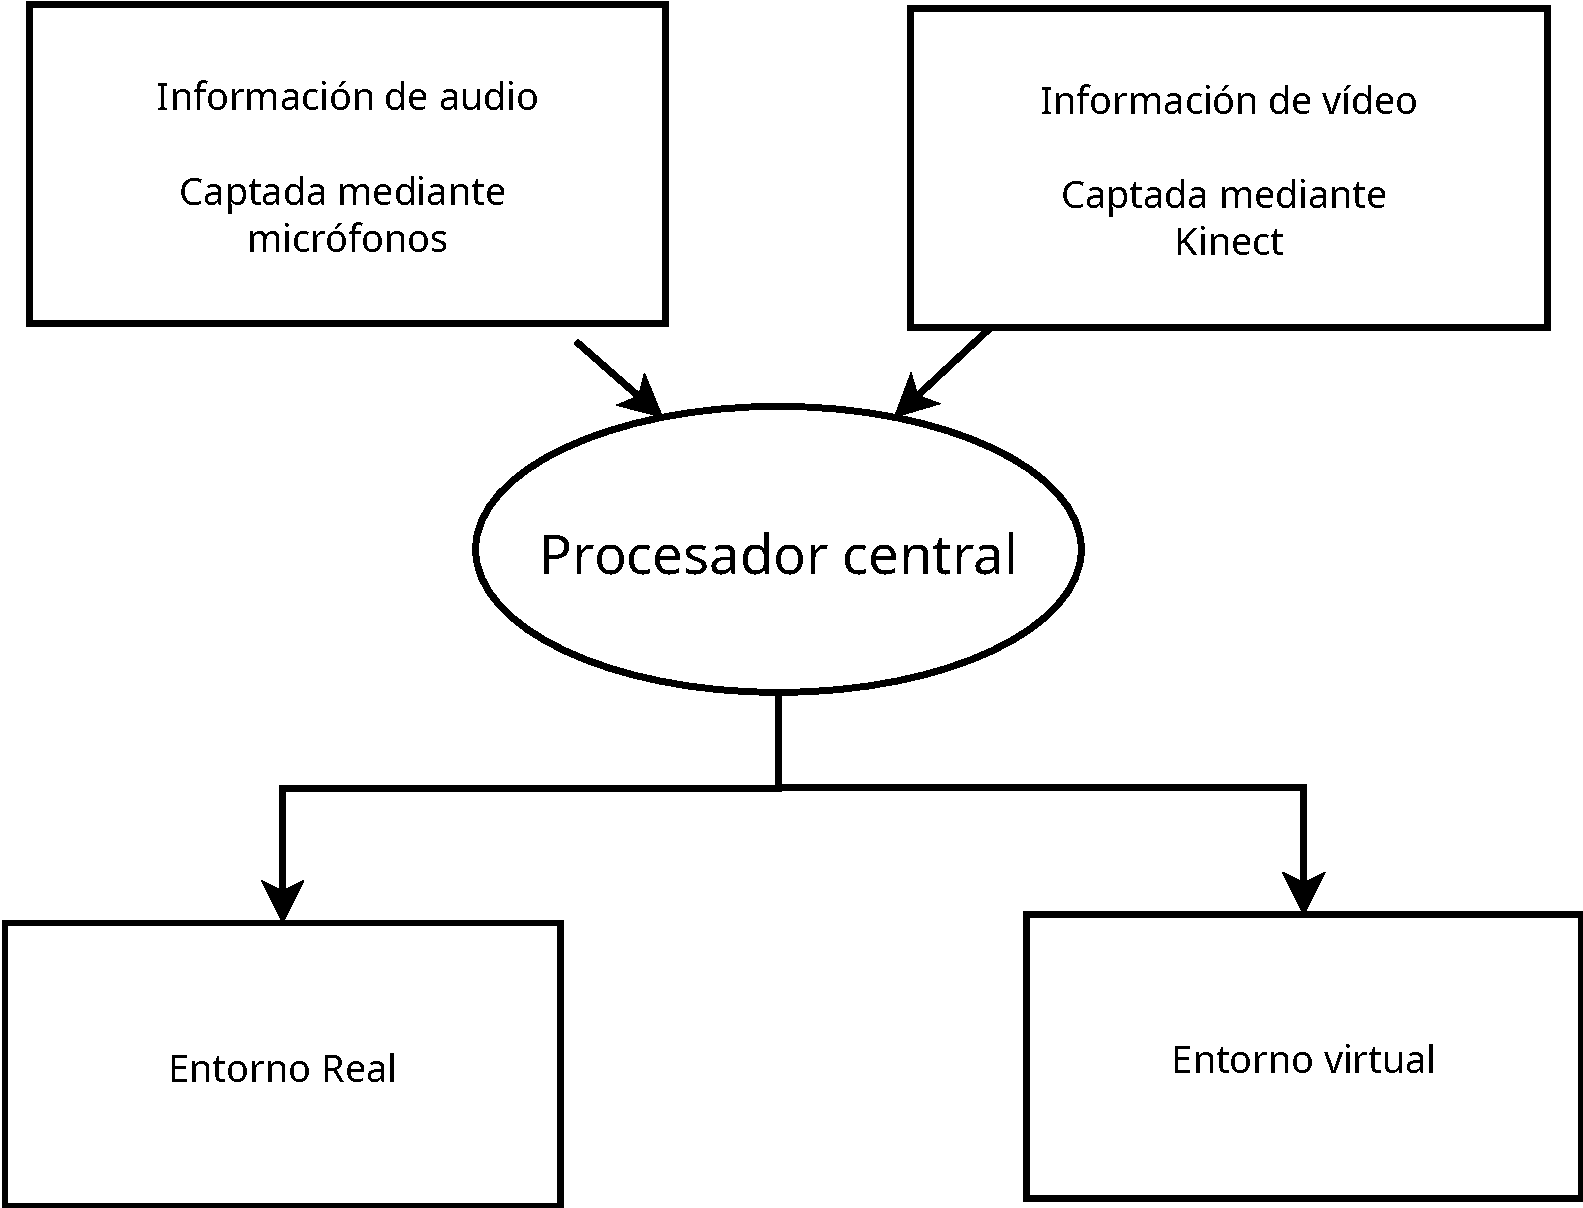
\includegraphics[width=3in]{Diagrama2.pdf}
%   \caption{Arquitectura del sistema experimental.}
%   \label{fig:arquitectura}
% \end{figure}


\section{Metodología y plan de trabajo}
\label{sec:metodologia-y-plan}

El trabajo seguirá un enfoque incremental, con las siguientes etapas,
orientadas a la consecución de los objetivos descritos en la
sección~\ref{sec:objetivos-y-campo}:

\begin{enumerate}
\item Lectura de los artículos sobre JoularJX y de la literatura sobre
  consumo energético del software.

\item Instalación de JoularJX y de Power Monitor for Windows, y
  verificación del entorno con un programa de prueba.

\item Estudio de las arquitecturas de Jackson y Gson, y diseño del banco
  de pruebas con JMH.

\item Ejecución de las mediciones con JoularJX, repetición para
  verificar su estabilidad y análisis de los resultados.

\item Comparación normalizada, evaluación de las limitaciones de
  JoularJX y extracción de conclusiones.

\item Redacción de la memoria final del TFG.
\end{enumerate}

El diagrama de Gantt asociado a esa planificación, para la convocatoria
de junio/julio de 2027, es el mostrado en la
figura~\ref{fig:diagrama-gantt}.

\begin{figure}[H]
  \centering

  \begin{ganttchart}[
    title height=1,
    x unit=0.045cm, % Ajusta el ancho del diagrama
    y unit title=0.6cm,
    y unit chart=0.5cm,
    group height=0.5,
    bar height=0.5,
    vgrid={*{6}{draw=none}, *1{draw, dotted}},
    hgrid,
    time slot format=isodate,
    group label font=\bfseries\footnotesize,
    bar label font=\footnotesize,
    title label font=\tiny,
    group/.append style={fill=gray!75},
    group peaks height=0.3,
    group peaks width=2,
    group peaks tip position=0,
    ]{2026-10-01}{2027-06-30}

    % Meses
    \gantttitlecalendar{year, month} \\

    % Tareas
    \ganttbar{Lecturas y estado del arte}{2026-10-01}{2026-11-30} \\
    \ganttbar{Instalación y configuración}{2026-11-01}{2026-12-31} \\
    \ganttbar{Diseño del banco de pruebas}{2027-01-01}{2027-01-31} \\
    \ganttbar{Experimentación y análisis}{2027-02-01}{2027-03-31} \\
    \ganttbar{Redacción de la memoria}{2027-04-01}{2027-05-31} \\
    \ganttbar{Revisión final y defensa}{2027-06-01}{2027-06-30}
  \end{ganttchart}
  \caption{Diagrama de Gantt de la planificación del trabajo.}
  \label{fig:diagrama-gantt}

\end{figure}


\section{Medios}
\label{sec:medios}

Las herramientas y recursos necesarios para desarrollar este proyecto
son los siguientes:

\begin{itemize}
\item Ordenador personal con Windows~11 y procesador Intel o AMD (a
  partir de Ryzen), con soporte de RAPL.

\item JDK~11 o superior y Apache Maven.

\item JoularJX (agente Java, licencia GPL-3.0)~\cite{joularjxrepo}.

\item Power Monitor for Windows, para la lectura de los contadores RAPL
  en Windows~\cite{winpowermonitor}.

\item Jackson Databind (FasterXML, Apache~2.0)~\cite{jackson} y Gson
  (Google, Apache~2.0)~\cite{gson}, disponibles en Maven Central.

\item Procesador de textos \LaTeX{} para la redacción de la memoria.

\item Repositorio Git para el control de versiones del código y de la
  documentación.

\item Acceso a las bases de datos bibliográficas de la UAH (IEEE Xplore,
  ACM Digital Library y ScienceDirect).
\end{itemize}

No se requieren medios hardware específicos ni financiación adicional.




% 
% END Normal sections. Edit/modify all within this section
%%%%%%%%%%%%%%%%%%%%%%%%%%%%%%%%%%%%%%%%%%%%%%%%%%%%%%%%%%%%%%%%%%%%%%%%%%% 
%%%%%%%%%%%%%%%%%%%%%%%%%%%%%%%%%%%%%%%%%%%%%%%%%%%%%%%%%%%%%%%%%%%%%%%%%%% 
%%%%%%%%%%%%%%%%%%%%%%%%%%%%%%%%%%%%%%%%%%%%%%%%%%%%%%%%%%%%%%%%%%%%%%%%%%% 
%%%%%%%%%%%%%%%%%%%%%%%%%%%%%%%%%%%%%%%%%%%%%%%%%%%%%%%%%%%%%%%%%%%%%%%%%%% 
%%%%%%%%%%%%%%%%%%%%%%%%%%%%%%%%%%%%%%%%%%%%%%%%%%%%%%%%%%%%%%%%%%%%%%%%%%% 
%%%%%%%%%%%%%%%%%%%%%%%%%%%%%%%%%%%%%%%%%%%%%%%%%%%%%%%%%%%%%%%%%%%%%%%%%%% 
%%%%%%%%%%%%%%%%%%%%%%%%%%%%%%%%%%%%%%%%%%%%%%%%%%%%%%%%%%%%%%%%%%%%%%%%%%% 


%%%%%%%%%%%%%%%%%%%%%%%%%%%%%%%%%%%%%%%%%%%%%%%%%%%%%%%%%%%%%%%%%%%%%%%%%%% 
% Bibliography
%%%%%%%%%%%%%%%%%%%%%%%%%%%%%%%%%%%%%%%%%%%%%%%%%%%%%%%%%%%%%%%%%%%%%%%%%%% 
\input{../Book/biblio/bibliography.tex}               % EDIT this file if required



\end{document}

